\chapter{Функции нескольких переменных: градиент, дифференциал и якобиан}\label{chap:multivariable}\markright{Глава 33}

\section{Область определения, линии уровня и предел}
\begin{definition}\term{Функция нескольких переменных} (\emph{multivariable function}) \(f:U\subseteq\mathbb R^n\to\mathbb R\) сопоставляет одному набору координат одно число. \par\term{Множество уровня} (\emph{level set}) имеет вид \(\{x\in U:f(x)=c\}\). В двух переменных это обычно линии уровня, в трёх — поверхности уровня.\end{definition}
\par\addvspace{5pt}\begin{lrbox}{\CatFlowBox}\begin{minipage}[t]{\linewidth}
\setlength{\parskip}{5pt}\setlength{\columnsep}{4.5mm}\setlength{\intextsep}{0pt}
\begin{wrapfigure}[9]{r}{54mm}

\includegraphics[width=54mm,height=58mm,keepaspectratio]{images/unique/art-148.png}
\end{wrapfigure}
Значение температуры в комнате зависит от трёх координат, а высота рельефа — от двух. Линия уровня объединяет точки с одним значением функции. Если перемещаться вдоль такой линии, значение сохраняется, хотя координаты меняются. Чтобы понять изменение в другом направлении, одного графика на плоскости уже недостаточно: нужны частные производные и полный дифференциал.
\par\WFclear\end{minipage}\end{lrbox}%
\ifdim\dimexpr\ht\CatFlowBox+\dp\CatFlowBox\relax<64mm\dp\CatFlowBox=\dimexpr64mm-\ht\CatFlowBox\relax\fi%
\noindent\usebox{\CatFlowBox}\par\addvspace{5pt}
\begin{definition}\term{Предел функции нескольких переменных} (\emph{multivariable limit}) \(f(x)\to L\) при \(x\to a\) означает: для любого \(\varepsilon>0\) найдётся \(\delta>0\), такое что \(x\in U\), \(0<\|x-a\|<\delta\) влечёт \(|f(x)-L|<\varepsilon\). Точка \(a\) должна быть предельной точкой \(U\).\end{definition}
\begin{definition}\term{Непрерывность} (\emph{continuity}) в \(a\in U\) означает, что для любого \(\varepsilon>0\) существует \(\delta>0\), при котором \(\|x-a\|<\delta\), \(x\in U\), влечёт \(|f(x)-f(a)|<\varepsilon\).\end{definition}
Проверка двух путей может опровергнуть существование предела, если ответы различаются. Совпадение результатов на нескольких путях предела не доказывает. Например, \(\frac{xy}{x^2+y^2}\) стремится к нулю вдоль обеих осей, но вдоль \(y=x\) равно \(\frac12\).
\section{Частные производные и дифференциал}
\begin{definition}\term{Частная производная} (\emph{partial derivative}) по \(x_j\) в открытой области определяется как обычная производная при фиксированных остальных координатах:
\[
\frac{\partial f}{\partial x_j}(a)
=\lim_{t\to0}\frac{f(a+te_j)-f(a)}t.
\]
Также пишут \(\partial_jf(a)\), \(f_{x_j}(a)\).
\end{definition}
\begin{definition}\term{Дифференцируемость} (\emph{total differentiability}) в \(a\) означает существование линейной функции \(L(h)\), для которой
\[
f(a+h)=f(a)+L(h)+r(h),\qquad
\lim_{h\to0,\ h\ne0}\frac{r(h)}{\|h\|}=0.
\]
\term{Дифференциал} (\emph{differential}) — линейная часть \(df_a(h)=L(h)\).
\end{definition}
\begin{definition}\term{Градиент} (\emph{gradient}) — вектор \(\nabla f=(\partial_1f,\ldots,\partial_nf)\). Если \(f\) дифференцируема, то \(df_a(h)=\langle\nabla f(a),h\rangle\).\end{definition}
\begin{theorem}[Непрерывные частные производные]
Если все частные производные существуют в окрестности \(a\) и непрерывны в \(a\), то \(f\) дифференцируема в \(a\). Одна дифференцируемость влечёт непрерывность и существование частных производных, но существования частных производных недостаточно.
\end{theorem}
\begin{proof}Для малого \(h\) изменяем координаты по одной, оставаясь в шаре внутри области. Разность \(f(a+h)-f(a)\) раскладывается в сумму \(n\) приращений одной переменной. По Лагранжу каждое равно \(\partial_jf(\xi_j)h_j\), где \(\xi_j\to a\) при \(h\to0\). Вычтем \(\sum_j\partial_jf(a)h_j\). Модуль остатка не больше \(\|h\|\sum_j|\partial_jf(\xi_j)-\partial_jf(a)|=o(\|h\|)\). Здесь \(r(h)=o(\|h\|)\) — краткая запись предельного условия из определения. Обратно, в определении дифференцируемости \(L(h)\to0\), что даёт непрерывность; подстановка \(h=te_j\) даёт частные производные и коэффициенты \(L\). Контрпример к достаточности одних частных производных разобран в задачах.\end{proof}
\begin{definition}\term{Производная по направлению} (\emph{directional derivative}) единичного вектора \(u\) — предел \(D_uf(a)=\lim_{t\to0}\frac{f(a+tu)-f(a)}t\), если он существует.\end{definition}
\begin{theorem}[Направление наибольшего роста]
Для дифференцируемой \(f\): \(D_uf(a)=\langle\nabla f(a),u\rangle\). Если \(\nabla f(a)\ne0\), наибольшая производная по единичному направлению равна \(\|\nabla f(a)\|\) и достигается при \(u=\frac{\nabla f(a)}{\|\nabla f(a)\|}\).
\end{theorem}
\par\addvspace{5pt}\begin{lrbox}{\CatFlowBox}\begin{minipage}[t]{\linewidth}
\setlength{\parskip}{5pt}\setlength{\columnsep}{4.5mm}\setlength{\intextsep}{0pt}
\begin{wrapfigure}[9]{l}{54mm}
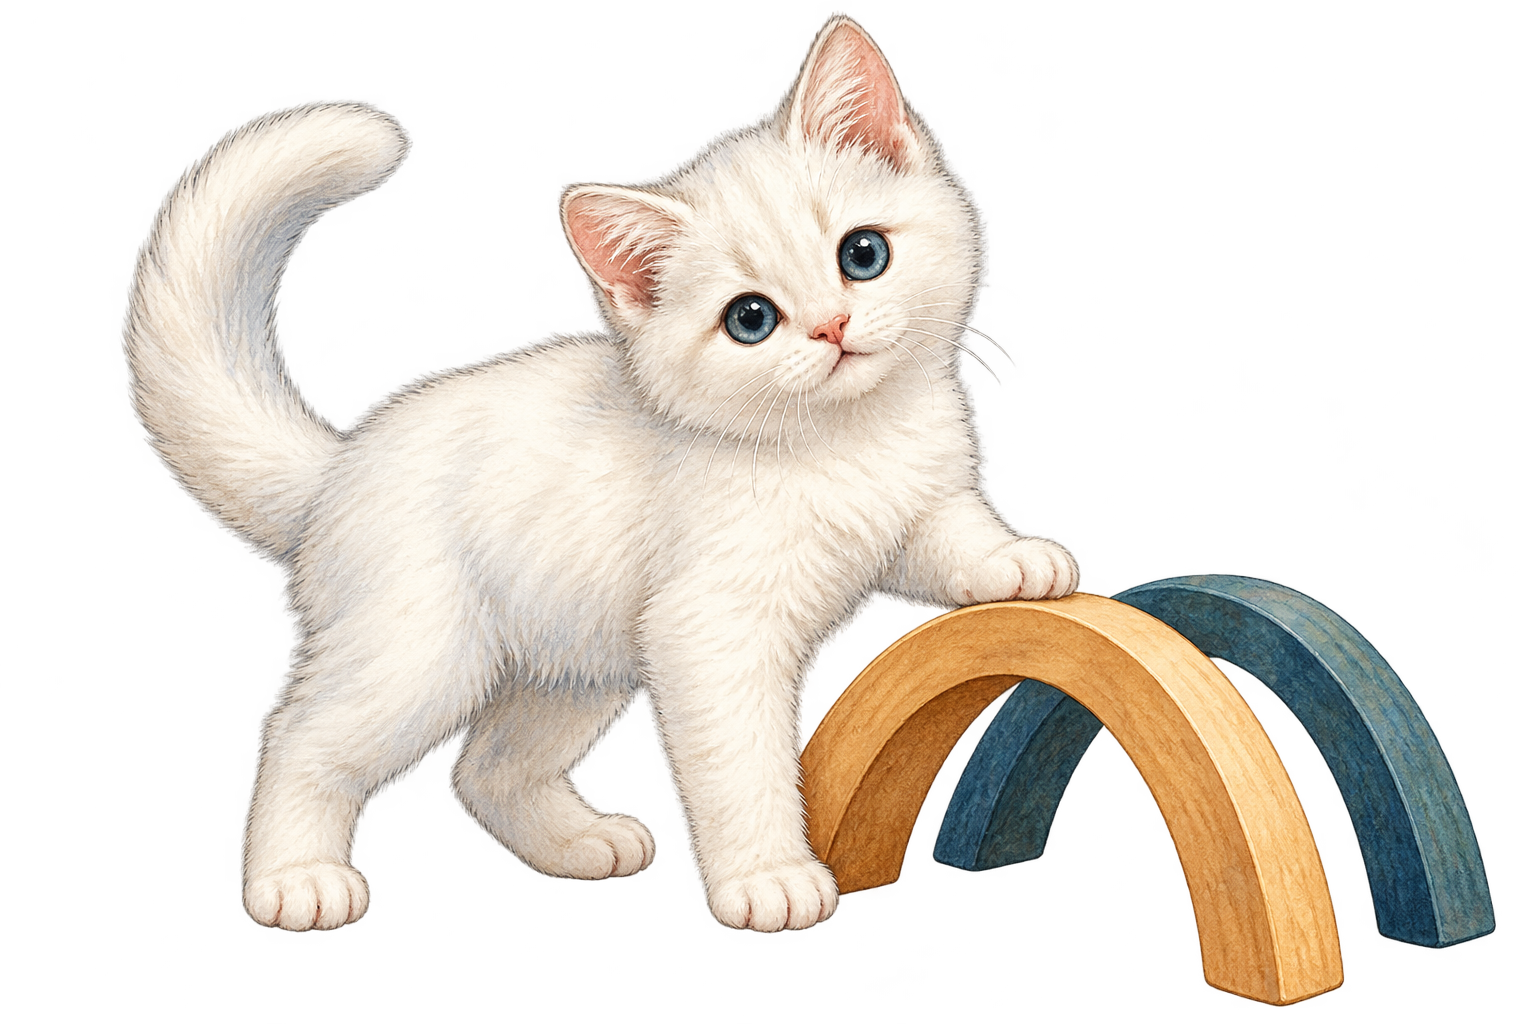
\includegraphics[width=54mm,height=58mm,keepaspectratio]{images/unique/art-151.png}
\end{wrapfigure}
\textit{Доказательство.} Подставляем \(h=tu\) в определение дифференцируемости. Остаток после деления на \(t\) стремится к нулю. Затем применяем неравенство Коши — Буняковского; указанное направление даёт равенство. При нулевом градиенте все производные по направлениям равны нулю.\hfill\(\blacksquare\)
\par\WFclear\end{minipage}\end{lrbox}%
\ifdim\dimexpr\ht\CatFlowBox+\dp\CatFlowBox\relax<64mm\dp\CatFlowBox=\dimexpr64mm-\ht\CatFlowBox\relax\fi%
\noindent\usebox{\CatFlowBox}\par\addvspace{5pt}

\par\addvspace{5pt}\begin{lrbox}{\CatFlowBox}\begin{minipage}[t]{\linewidth}
\setlength{\parskip}{5pt}\setlength{\columnsep}{4.5mm}\setlength{\intextsep}{0pt}
\begin{wrapfigure}[11]{l}{54mm}
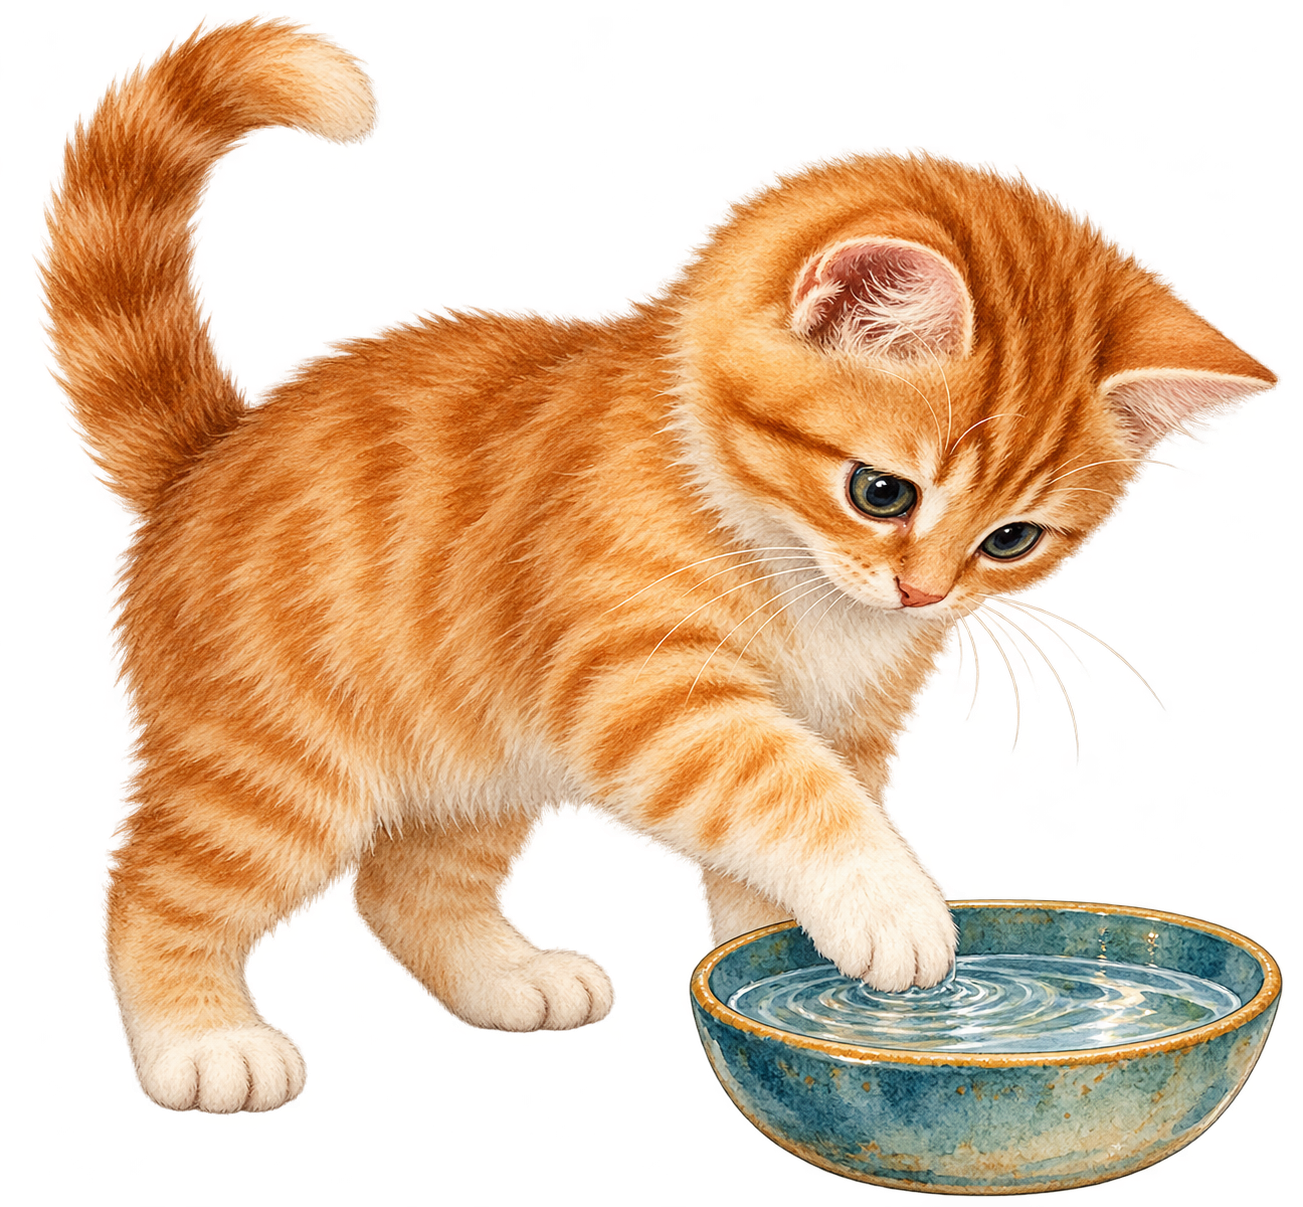
\includegraphics[width=54mm,height=58mm,keepaspectratio]{images/unique/art-149.png}
\end{wrapfigure}
Градиент описывает локальное изменение, а не обещает добраться до глобального максимума. В точке с нулевым градиентом может быть минимум, максимум или седло. Например, у \(x^2+y^2\) в нуле минимум, а у \(x^2-y^2\) значение растёт вдоль одной оси и убывает вдоль другой. Оба градиента в нуле одинаковы.
\par\WFclear\end{minipage}\end{lrbox}%
\ifdim\dimexpr\ht\CatFlowBox+\dp\CatFlowBox\relax<64mm\dp\CatFlowBox=\dimexpr64mm-\ht\CatFlowBox\relax\fi%
\noindent\usebox{\CatFlowBox}\par\addvspace{5pt}
\begin{definition}\term{Касательная плоскость к графику} (\emph{tangent plane}) дифференцируемой \(z=f(x,y)\) в \((a,b,f(a,b))\) задаётся
\[
z=f(a,b)+f_x(a,b)(x-a)+f_y(a,b)(y-b).
\]
\end{definition}
\section{Якобиан и правило цепочки}
\begin{definition}\term{Дифференцируемость векторного отображения} (\emph{differentiability of a vector-valued map}) \(F:U\subseteq\mathbb R^n\to\mathbb R^m\) в \(a\in U\), где \(U\) открыто, означает \(F(a+h)=F(a)+Mh+r(h)\), \(\|r(h)\|/\|h\|\to0\), для некоторого линейного отображения \(M\). Это равносильно дифференцируемости всех компонент; матрица \(M\) в стандартных базисах состоит из их частных производных.\end{definition}
\begin{definition}\term{Матрица Якоби} (\emph{Jacobian matrix}) отображения \(F:\mathbb R^n\supset U\to\mathbb R^m\) состоит из \( (DF)_{ij}=\partial_jF_i\). \par\term{Якобиан преобразования} (\emph{Jacobian determinant}) при \(m=n\) — число \(\det DF\). Матрицу и её определитель нужно различать.\end{definition}
Для квадратной матрицы любого порядка определитель можно определить рекурсивно: для \(1\times1\) это её единственный элемент, а для \(n\times n\)
\[
\det A=\sum_{j=1}^n(-1)^{1+j}a_{1j}\det A_{1j},
\]
где \(A_{1j}\) получается удалением первой строки и \(j\)-го столбца. При \(n=2\) получается \(ad-bc\). При \(n=3\) это та же формула, что в смешанном произведении.
\begin{theorem}[Многомерное правило цепочки]
Если \(G\) дифференцируема в \(a\), а \(F\) — в \(G(a)\), то \(F\circ G\) дифференцируема и
\[
D(F\circ G)(a)=DF(G(a))\,DG(a).
\]
\end{theorem}
\begin{proof}Запишем \(G(a+h)-G(a)=Mh+o(\|h\|)\), а \(F(G(a)+k)-F(G(a))=Lk+o(\|k\|)\). Первое равенство даёт \(k=O(\|h\|)\): его норма не больше некоторой постоянной, умноженной на \(\|h\|\). После подстановки получаем \(LMh+o(\|h\|)\). Это и есть дифференцируемость композиции с матрицей \(LM\).\end{proof}
\par\addvspace{5pt}\begin{lrbox}{\CatFlowBox}\begin{minipage}[t]{\linewidth}
\setlength{\parskip}{5pt}\setlength{\columnsep}{4.5mm}\setlength{\intextsep}{0pt}
\begin{wrapfigure}[11]{r}{54mm}
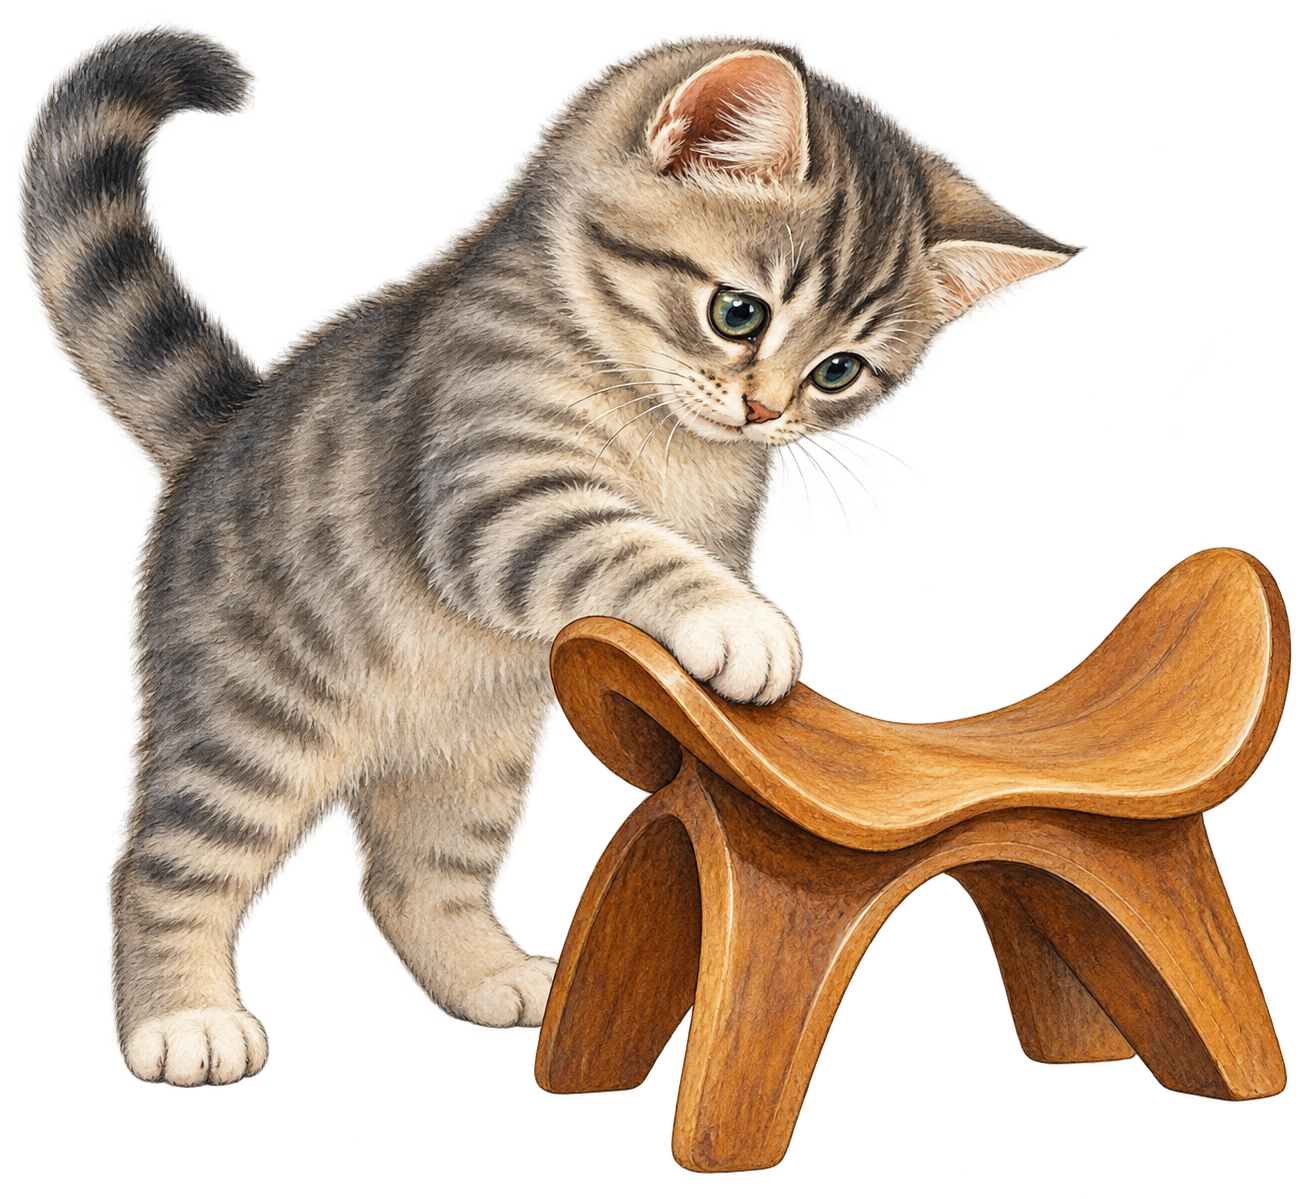
\includegraphics[width=54mm,height=58mm,keepaspectratio]{images/unique/art-150.png}
\end{wrapfigure}
Якобиан измеряет локальный коэффициент изменения ориентированного объёма. Для площади и объёма при интегрировании нужен его модуль. Ненулевой якобиан не гарантирует взаимной однозначности преобразования на всей области. Например, \((u,v)\mapsto(u^2-v^2,2uv)\) имеет якобиан \(4(u^2+v^2)\), но точки \((u,v)\) и \((-u,-v)\) дают один образ.
\par\WFclear\end{minipage}\end{lrbox}%
\ifdim\dimexpr\ht\CatFlowBox+\dp\CatFlowBox\relax<64mm\dp\CatFlowBox=\dimexpr64mm-\ht\CatFlowBox\relax\fi%
\noindent\usebox{\CatFlowBox}\par\addvspace{5pt}
\section{Вторые производные и экстремумы}
\begin{definition}\term{Класс \(C^k\)} (\emph{class \(C^k\)}) состоит из функций с непрерывными частными производными всех порядков до \(k\) включительно. \par\term{Гессиан} (\emph{Hessian matrix}) функции \(f\in C^2\) — матрица \(H_f=(\partial_i\partial_jf)\).\end{definition}
\begin{theorem}[Равенство смешанных производных; Clairaut's theorem]
У функции класса \(C^2\) выполнено \(f_{xy}=f_{yx}\); аналогично для любой пары координат в \(\mathbb R^n\).
\end{theorem}
\begin{proof}Возьмём прямоугольное приращение \(f(a+h,b+k)-f(a+h,b)-f(a,b+k)+f(a,b)\). Дважды применяя основную теорему анализа, сначала по одной координате, затем по другой, выражаем его как повторный интеграл \(f_{xy}\). При обратном порядке рассуждения получаем повторный интеграл \(f_{yx}\). Делим оба выражения на \(hk\). При \(h,k\to0\) непрерывность подынтегральных функций даёт соответственно \(f_{xy}(a,b)\) и \(f_{yx}(a,b)\). Исходная разность одинакова, поэтому пределы равны; перестановка порядка интегрирования здесь не используется.\end{proof}
\begin{theorem}[Критическая точка и квадратичная часть в двух переменных]
Во внутренней точке локального экстремума дифференцируемой функции \(\nabla f=0\). Если \(f\in C^2\), \(\nabla f(a)=0\) и \(H_f(a)\) положительно определена, в \(a\) строгий локальный минимум; при отрицательной определённости — строгий локальный максимум. При неопределённости имеется седло. Полуопределённость сама по себе ответа не даёт.
\end{theorem}
\begin{proof}Ограничение на каждую координатную прямую имеет экстремум; теорема Ферма даёт нулевые частные производные. Для малых \(h\) применим интегрирование по частям к \(g(t)=f(a+th)\):
\[
f(a+h)-f(a)-\langle\nabla f(a),h\rangle
=\int_0^1(1-t)h^{\mathrm T}H_f(a+th)h\,dt.
\]
Непрерывность гессиана даёт \(\frac12h^{\mathrm T}H_f(a)h+o(\|h\|^2)\). В двух переменных положительно определённая симметричная матрица имеет два положительных собственных значения, поэтому её форма не меньше \(\lambda_{\min}\|h\|^2\). Остаток этого знака не меняет при достаточно малом \(h\ne0\). Для отрицательной формы рассматриваем \(-f\). При разных знаках собственных значений выбираем два собственных направления; приращения имеют разные знаки. Примеры \(x^4+y^4\), \(x^4-y^4\) имеют один нулевой гессиан, но разное поведение.\end{proof}
\begin{definition}\term{Векторное поле} (\emph{vector field}) на \(U\subseteq\mathbb R^n\) — отображение \(F:U\to\mathbb R^n\). Например, поле скоростей приписывает каждой точке вектор направления и величины скорости.\end{definition}

\par\noindent\begin{minipage}{\linewidth}\section*{Графики}
\begin{center}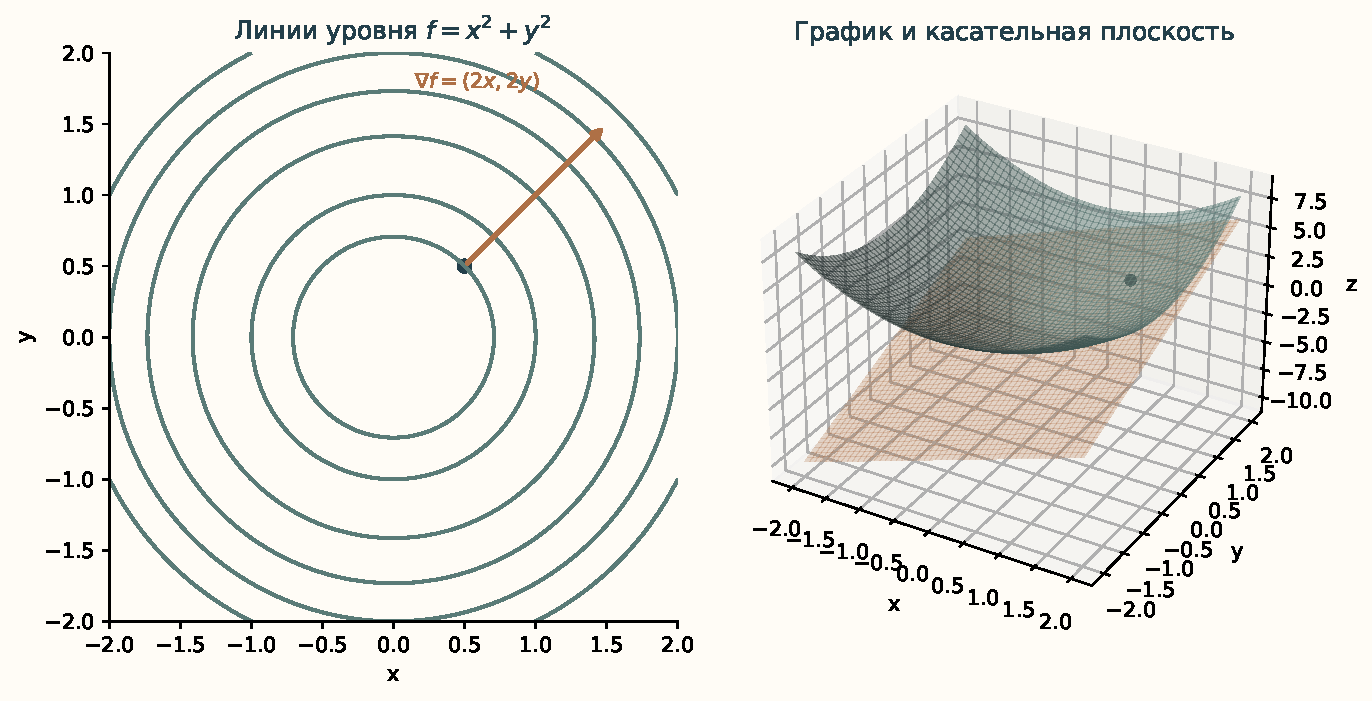
\includegraphics[width=\textwidth,height=.79\textheight,keepaspectratio]{images/atlas-multivariable.pdf}\par\small Линии уровня, градиент и касательная плоскость\end{center}\end{minipage}\par
\Needspace{7\baselineskip}\section*{Задачи}
\begingroup\setlength{\parskip}{0pt}
\noindent\begin{minipage}[t]{\linewidth}\textbf{33.1.} Найди область определения \(f(x,y)=\sqrt{1-x^2-y^2}\) и опиши её границу.\par\end{minipage}\par
\noindent\begin{minipage}[t]{\linewidth}\textbf{33.2.} Нарисуй линии уровня \(x^2+y^2=c\) при \(c=-1,0,1,4\).\par\end{minipage}\par
\noindent\begin{minipage}[t]{\linewidth}\textbf{33.3.} Докажи, что \(\dfrac{xy}{x^2+y^2}\) не имеет предела в нуле.\par\end{minipage}\par
\noindent\begin{minipage}[t]{\linewidth}\textbf{33.4.} Найди \(f_x,f_y\) для \(f(x,y)=x^2y+\sin y\).\par\end{minipage}\par
\noindent\begin{minipage}[t]{\linewidth}\textbf{33.5.} Найди градиент \(f=x^2+y^2\) в точке \((1,2)\).\par\end{minipage}\par
\par\addvspace{2pt}\begin{lrbox}{\CatFlowBox}\begin{minipage}[t]{\linewidth}
\setlength{\parskip}{1pt}\setlength{\columnsep}{4.5mm}\setlength{\intextsep}{0pt}
\begin{wrapfigure}[13]{r}{54mm}

\includegraphics[width=54mm,height=58mm,keepaspectratio]{images/unique/art-152.png}
\end{wrapfigure}
\textbf{33.6.} Для той же функции и точки найди производную по единичному направлению \((\dfrac35,\dfrac45)\).\par

\textbf{33.7.} Укажи единичное направление наибольшего роста \(x^2+y^2\) в \((1,2)\) и саму наибольшую производную.\par

\textbf{33.8.} Построй касательную плоскость к \(z=x^2+y^2\) при \(x=1,y=2\).\par

\textbf{33.9.} Приблизь изменение \(f(x,y)=xy\) от \((2,3)\) к \((2{,}01,2{,}98)\) дифференциалом; найди также точное изменение.\par
\par\WFclear\end{minipage}\end{lrbox}%
\ifdim\dimexpr\ht\CatFlowBox+\dp\CatFlowBox\relax<58mm\dp\CatFlowBox=\dimexpr58mm-\ht\CatFlowBox\relax\fi%
\noindent\usebox{\CatFlowBox}\par\addvspace{2pt}

\noindent\begin{minipage}[t]{\linewidth}\textbf{33.10.} Найди матрицу Якоби и её определитель для \(F(u,v)=(u+2v,3u-v)\).\par\end{minipage}\par
\noindent\begin{minipage}[t]{\linewidth}\textbf{33.11.} Для \(F(u,v)=(u^2-v^2,2uv)\) найди якобиан и объясни, почему \(F\) не инъективно вне нуля.\par\end{minipage}\par
\noindent\begin{minipage}[t]{\linewidth}\textbf{33.12.} Для полярного преобразования \(x=r\cos\theta,y=r\sin\theta\) найди якобиан по \(r,\theta\).\par\end{minipage}\par
\noindent\begin{minipage}[t]{\linewidth}\textbf{33.13.} Найди частные производные \(f(x,y,z)=xyz\).\par\end{minipage}\par
\noindent\begin{minipage}[t]{\linewidth}\textbf{33.14.} Температурная модель \(T(x,y)=20-x^2-2y^2\). Найди градиент при \((1,1)\) и направление наибольшего уменьшения.\par\end{minipage}\par
\noindent\begin{minipage}[t]{\linewidth}\textbf{33.15.} Путь задан \(x(t)=t,y(t)=t^2\); \(f(x,y)=x^2+y\). Найди \(\dfrac d{dt}f(x(t),y(t))\) двумя способами.\par\end{minipage}\par
\noindent\begin{minipage}[t]{\linewidth}\textbf{33.16.} Найди гессиан \(f(x,y)=x^2+3xy+2y^2\) и классифицируй критическую точку.\par\end{minipage}\par
\noindent\begin{minipage}[t]{\linewidth}\textbf{33.17.} Классифицируй нуль для \(x^2+2y^2\), \(-x^2-y^2\), \(x^2-y^2\).\par\end{minipage}\par
\noindent\begin{minipage}[t]{\linewidth}\textbf{33.18.} Почему нулевой гессиан не позволяет классифицировать нуль у \(x^4+y^4\) и \(x^4-y^4\)?\par\end{minipage}\par
\noindent\begin{minipage}[t]{\linewidth}\textbf{33.19.}\starmark{} Функция равна \(\dfrac{xy}{\sqrt{x^2+y^2}}\) вне нуля и \(0\) в нуле. Найди частные производные в нуле и докажи отсутствие дифференцируемости.\par\end{minipage}\par
\noindent\begin{minipage}[t]{\linewidth}\textbf{33.20.}\starmark{} Пусть \(f\) дифференцируема в точках рассматриваемой кривой. Докажи: если дифференцируемая кривая \(\gamma(t)\) лежит на уровне \(f=c\), то \(\nabla f(\gamma(t))\) перпендикулярен \(\gamma^{\prime}(t)\).\par\end{minipage}\par
\noindent\begin{minipage}[t]{\linewidth}\textbf{33.21.}\starmark{} Докажи, что \(\nabla f=0\) на выпуклой открытой области влечёт постоянство \(f\), если \(f\) дифференцируема.\par\end{minipage}\par
\noindent\begin{minipage}[t]{\linewidth}\textbf{33.22.}\starmark{} При каких \(x,y\) матрица Якоби \(F(x,y)=(e^x\cos y,e^x\sin y)\) невырождена? Является ли \(F\) глобально инъективным?\par\end{minipage}\par
\noindent\begin{minipage}[t]{\linewidth}\textbf{33.23.} Найди якобиан \(F(x,y,z)=(2x,3y,4z)\) и коэффициент изменения объёма.\par\end{minipage}\par
\noindent\begin{minipage}[t]{\linewidth}\textbf{33.24.} Вычисли определитель \(\begin{pmatrix}1&2&0\\0&3&1\\2&0&4\end{pmatrix}\) разложением по первой строке.\par\end{minipage}\par
\endgroup
